\documentclass[aspectratio=169]{beamer}

\usepackage{amsmath, amssymb}
\usepackage{tikz}
\usepackage{booktabs}
\usepackage{xcolor}
\usepackage{graphicx}
\usepackage{colortbl}

\usetikzlibrary{arrows.meta, positioning, calc, shapes.geometric}

\usefonttheme{professionalfonts}
\setbeamertemplate{navigation symbols}{}

% --- Color theme (white/professional) ---
\definecolor{darktext}{HTML}{1A1A2E}
\definecolor{accent}{HTML}{2D3494}
\definecolor{accentblue}{HTML}{1565C0}
\definecolor{accentgreen}{HTML}{2E7D32}
\definecolor{accentred}{HTML}{C62828}
\definecolor{accentorange}{HTML}{E65100}
\definecolor{accentteal}{HTML}{00695C}
\definecolor{midgray}{HTML}{555555}
\definecolor{lightgray}{HTML}{999999}
\definecolor{boxfill}{HTML}{F0F2F8}
\definecolor{boxfillgreen}{HTML}{EDF7ED}
\definecolor{boxfillred}{HTML}{FDECEC}
\definecolor{boxfillorange}{HTML}{FFF3E0}
\definecolor{boxfillblue}{HTML}{E8EAF6}

\setbeamercolor{background canvas}{bg=white}
\setbeamercolor{normal text}{fg=darktext}
\setbeamercolor{frametitle}{fg=accent}
\setbeamercolor{itemize item}{fg=accent}
\setbeamercolor{itemize subitem}{fg=accentblue}

\setbeamertemplate{itemize item}{\textbullet}
\setbeamertemplate{itemize subitem}{--}

\setbeamersize{text margin left=8mm, text margin right=8mm}

% --- page number ---
\setbeamertemplate{footline}{%
    \raisebox{8pt}{\makebox[\paperwidth]{\hfill\makebox[6em]{\color{lightgray}\small\texttt{\insertframenumber/\inserttotalframenumber}}}}%
}

% --- Custom commands ---
\newcommand{\accentline}{\vspace{1pt}{\color{accent}\rule{0.3\textwidth}{1.5pt}}\vspace{4pt}}
\newcommand{\resultbox}[3][boxfill]{%
    \begin{tikzpicture}
    \node[fill=#1, rounded corners=3pt, draw=#2, line width=0.8pt, text width=\linewidth-16pt, inner sep=6pt, text=darktext] {#3};
    \end{tikzpicture}%
}

\title{}
\author{}
\date{}

\begin{document}

% ============================================================
% SLIDE 1: Title
% ============================================================
\begin{frame}[plain]
    \vspace{1.8cm}
    \begin{center}
        {\color{accent}\rule{0.5\textwidth}{1.5pt}}\\[10pt]
        {\LARGE\bfseries\color{darktext} Targeted Lobbying on\\[4pt] Council Networks}\\[10pt]
        {\large\color{accentblue} Final Presentation}\\[20pt]
        {\color{midgray} Samir Kadariya \& Bryce Roberts}\\[4pt]
        {\small\color{lightgray} 14.18}
    \end{center}
\end{frame}

% ============================================================
% SLIDE 2: The puzzle
% ============================================================
\begin{frame}{Whom should a lobbyist target?}
\accentline
\vspace{6pt}
\begin{columns}[T]
    \begin{column}{0.58\textwidth}
        \vspace{12pt}
        {\large A lobbyist with a limited budget.}\\[14pt]
        {\large A council connected by party,\\ committee, and personal ties.}\\[14pt]
        {\large Pressure on one member spills\\ over to others.}
    \end{column}
    \begin{column}{0.40\textwidth}
        \begin{center}
        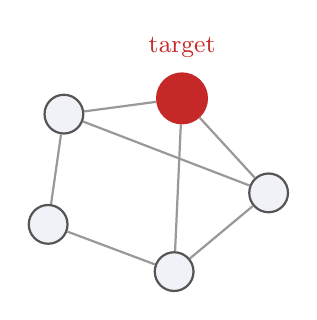
\begin{tikzpicture}[scale=1.0,
            nd/.style={circle, draw=midgray, fill=boxfill, line width=0.8pt, minimum size=14pt, inner sep=0pt},
            tg/.style={circle, draw=accentred, fill=accentred, line width=0.8pt, minimum size=18pt, inner sep=0pt}]
            \node[nd] (A) at (0,1.6) {};
            \node[tg] (B) at (1.5,1.8) {};
            \node[nd] (C) at (2.6,0.6) {};
            \node[nd] (D) at (1.4,-0.4) {};
            \node[nd] (E) at (-0.2,0.2) {};
            \draw[lightgray, line width=0.8pt] (A)--(B);
            \draw[lightgray, line width=0.8pt] (B)--(C);
            \draw[lightgray, line width=0.8pt] (C)--(D);
            \draw[lightgray, line width=0.8pt] (D)--(E);
            \draw[lightgray, line width=0.8pt] (E)--(A);
            \draw[lightgray, line width=0.8pt] (A)--(C);
            \draw[lightgray, line width=0.8pt] (B)--(D);
            \node[above=2pt, accentred, font=\small] at (B.north) {target};
        \end{tikzpicture}
        \end{center}
    \end{column}
\end{columns}
\end{frame}

% ============================================================
% SLIDE 3: What we keep from the literature
% ============================================================
\begin{frame}{What we keep from the literature}
\accentline
\vspace{6pt}

{\color{accentred}\bfseries Shleifer \& Vishny (1993).} {\small Bribes shift incentives. We keep this as the lobbyist effort $t_i$ in the payoff.}

\vspace{12pt}

{\color{accentgreen}\bfseries Galeotti, Golub \& Goyal (2020).} {\small Linear-quadratic network game; planner intervenes to maximize welfare.}

\vspace{12pt}

{\color{accent}\bfseries Our move.} {\small Swap welfare-maximization for \emph{minimum cost to pass a bill}. The problem becomes a linear program.}

\vspace{16pt}

\resultbox[boxfillblue]{accent}{%
    {\color{accent}\bfseries Old answer:} {\small eigenvector centrality.}\\[2pt]
    {\color{accent}\bfseries New answer:} {\small Katz--Bonacich centrality with decay $\beta/c$.}
}
\end{frame}

% ============================================================
% SLIDE 4: The model
% ============================================================
\begin{frame}{The model}
\accentline
\vspace{14pt}
\begin{center}
\[
    \boxed{\, U_i \;=\; a_i\!\left(b_i + t_i + \beta \sum_j g_{ij}\, a_j\right) \;-\; \tfrac{1}{2}\, c\, a_i^2 \,}
\]
\end{center}
\vspace{10pt}

{\small\color{accentred}\bfseries $b_i$:}\, baseline inclination toward the bill\\[6pt]
{\small\color{accent}\bfseries $t_i$:}\, lobbyist effort placed on member $i$\\[6pt]
{\small\color{accentgreen}\bfseries $\beta$, $c$:}\, peer-effect strength and own-action cost

\vspace{14pt}

{\small Lobbyist commits to $t \geq 0$, council picks $a$, bill passes if $\sum_i a_i \geq \bar T$.}
\end{frame}

% ============================================================
% SLIDE 5: Solving for a* --- best response
% ============================================================
\begin{frame}{Solving for the equilibrium: best response}
\accentline
\vspace{8pt}

{\small Each $U_i$ is strictly concave in $a_i$ (since $c > 0$), so the first-order condition is sufficient. Differentiate $U_i$ with respect to $a_i$:}

\vspace{2pt}
\[
    \frac{\partial U_i}{\partial a_i} \;=\; b_i \;+\; t_i \;+\; \beta \sum_{j \in N} g_{ij}\, a_j \;-\; c\, a_i \;=\; 0.
\]

{\small Solve for $a_i$ to get member $i$'s best response, given everyone else's actions:}

\vspace{2pt}
\[
    a_i \;=\; \frac{1}{c}\!\left(\, b_i \;+\; t_i \;+\; \beta \sum_{j \in N} g_{ij}\, a_j \,\right).
\]

\vspace{6pt}

{\small\color{midgray} Each member responds linearly to three things: their own preference, the lobbyist's push, and a peer-weighted average of neighbors' actions.}
\end{frame}

% ============================================================
% SLIDE 6: Solving for a* --- stack and invert
% ============================================================
\begin{frame}{Solving for the equilibrium}
\accentline
\vspace{8pt}

{\small Stack the $n$ best responses into vector form:}

\vspace{2pt}
\[
    c\,\mathbf{a} \;=\; (\mathbf{b} + \mathbf{t}) \;+\; \beta\, G\,\mathbf{a}
    \quad\Longleftrightarrow\quad
    (cI - \beta G)\,\mathbf{a} \;=\; \mathbf{b} + \mathbf{t}.
\]

{\small Under the spectral condition $c > \beta\,\lambda_{\max}(G)$, the matrix $cI - \beta G$ is positive definite, so it inverts cleanly:}

\vspace{2pt}
\[
    \boxed{\;a^*(t) \;=\; M\,(b + t), \qquad M \;:=\; (cI - \beta G)^{-1}\;}
\]

\vspace{6pt}

{\small\color{midgray} Strict concavity of each $U_i$ in $a_i$ makes this the unique Nash equilibrium of the council subgame.}
\end{frame}

% ============================================================
% SLIDE 7: Council equilibrium
% ============================================================
\begin{frame}{Council equilibrium}
\accentline
\vspace{8pt}

{\small Under the spectral-radius condition $c > \beta\,\lambda_{\max}(G)$, the council has a unique Nash equilibrium:}

\vspace{6pt}
\[
    a^*(t) \;=\; M\,(b + t), \qquad M \;:=\; (cI - \beta G)^{-1}.
\]
\vspace{4pt}

\resultbox[boxfillblue]{accent}{%
    {\color{accent}\bfseries Katz--Bonacich centrality with decay $\beta/c$:}\\[3pt]
    {$\displaystyle v \;:=\; M\mathbf{1}.$}
}

\vspace{10pt}

{\small\color{midgray} $v_i$ is the aggregate council support generated when the lobbyist places one unit of effort on member $i$ and zero on everyone else.}
\end{frame}

% ============================================================
% SLIDE 8: The lobbyist's LP
% ============================================================
\begin{frame}{The lobbyist's problem becomes an LP}
\accentline
\vspace{8pt}

{\small Aggregate support is linear in $t$:}
\[
    \textstyle\sum_i a_i^*(t) \;=\; v^\top b \;+\; v^\top t.
\]

\vspace{4pt}

\begin{center}
\[
    \boxed{\;\;\min_{t \geq 0} \;\mathbf{1}^\top t \quad\text{s.t.}\quad v^\top t \;\geq\; \Delta \;:=\; \bar T - v^\top b\;\;}
\]
\end{center}

\vspace{10pt}

{\small The whole game collapses to one linear constraint on the non-negative orthant.}
\end{frame}

% ============================================================
% SLIDE 9: Theorem 1 -- Concentration
% ============================================================
\begin{frame}{Theorem 1 --- Concentration}
\accentline
\vspace{8pt}

\resultbox[boxfillgreen]{accentgreen}{%
    {\color{accentgreen}\bfseries Theorem 1 (Concentration on max Katz--Bonacich).}\\[4pt]
    {\small Suppose $\Delta = \bar T - v^\top b > 0$ and let $i^* \in \arg\max_i v_i$. A cost-minimizing plan loads the entire budget on $i^*$, with}
    \[
        t^*_{i^*} \;=\; \frac{\Delta}{v_{i^*}}, \qquad t^*_j \;=\; 0 \;\;\forall j \neq i^*,
    \]
    {\small and minimum cost}
    \[
        C^*(\bar T) \;=\; \frac{\bar T - v^\top b}{\max_i v_i}.
    \]
}

\vspace{8pt}

{\small The lobbyist puts the \emph{whole} budget on the member with the highest Katz--Bonacich centrality. No spreading.}
\end{frame}

% ============================================================
% SLIDE 10: Proof of Theorem 1 --- lower bound
% ============================================================
\begin{frame}{Proof of Theorem 1: lower bound on cost}
\accentline
\vspace{8pt}

{\small Take any feasible $t \geq 0$ with $v^\top t \geq \Delta$. The constraint chains into a lower bound on the total spend:}

\vspace{2pt}
\[
    \Delta \;\leq\; v^\top t \;=\; \sum_{i \in N} v_i\, t_i \;\leq\; \max_i v_i \cdot \sum_{i} t_i \;=\; v_{i^*} \cdot \mathbf{1}^\top t.
\]

{\small Divide through by $v_{i^*}$:}

\vspace{2pt}
\[
    \boxed{\;\mathbf{1}^\top t \;\geq\; \frac{\Delta}{v_{i^*}}\;}
\]

\vspace{6pt}

{\small\color{midgray} No feasible plan can achieve cost below $\Delta$ divided by the maximum Katz--Bonacich centrality.}
\end{frame}

% ============================================================
% SLIDE 11: Proof of Theorem 1 --- achievability
% ============================================================
\begin{frame}{Proof of Theorem 1}
\accentline
\vspace{8pt}

{\small We now exhibit a feasible plan that hits the lower bound. Define $\hat t$ to put the entire budget on member $i^*$:}

\vspace{2pt}
\[
    \hat t \;:=\; \frac{\Delta}{v_{i^*}}\, e_{i^*}, \qquad \text{zero on every other member.}
\]

{\small Three quick checks:}
\vspace{2pt}
\begin{itemize}\setlength{\itemsep}{3pt}
    \item {\small \textbf{Non-negative.} $\hat t \geq 0$. \checkmark}
    \item {\small \textbf{Feasible.} $\;v^\top \hat t \;=\; v_{i^*} \cdot \dfrac{\Delta}{v_{i^*}} \;=\; \Delta$. \checkmark}
    \item {\small \textbf{Cost.} $\;\mathbf{1}^\top \hat t \;=\; \dfrac{\Delta}{v_{i^*}}$ --- matches the lower bound. \checkmark}
\end{itemize}

\vspace{6pt}

{\small\color{midgray} The all-on-$i^*$ corner achieves the floor, so it is optimal.\hfill$\blacksquare$}
\end{frame}

% ============================================================
% SLIDE 12: 3-path example -- setup
% ============================================================
\begin{frame}{A worked example: 3-member path}
\accentline
\vspace{8pt}

\begin{center}
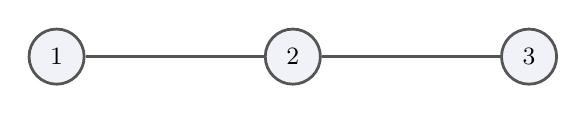
\begin{tikzpicture}[scale=1.0,
    nd/.style={circle, draw=midgray, fill=boxfill, line width=1pt, minimum size=0.7cm, inner sep=0pt, font=\small}]
    \node[nd] (n1) at (-3.0,0) {1};
    \node[nd] (n2) at (0,0) {2};
    \node[nd] (n3) at (3.0,0) {3};
    \draw[midgray, line width=1.2pt] (n1)--(n2);
    \draw[midgray, line width=1.2pt] (n2)--(n3);
\end{tikzpicture}
\end{center}

\vspace{12pt}

\begin{columns}[T]
    \begin{column}{0.45\textwidth}
        {\small\bfseries\color{accent} Parameters}\\[6pt]
        {\small $c \;=\; 1, \quad \beta \;=\; 0.4$}\\[4pt]
        {\small Baseline beliefs $b \;=\; \mathbf{0}$}\\[4pt]
        {\small Passage threshold $\bar T \;=\; 1$}
    \end{column}
    \begin{column}{0.50\textwidth}
        {\small\bfseries\color{accent} Adjacency matrix}\\[-2pt]
        \[
            G \;=\; \begin{pmatrix} 0 & 1 & 0 \\ 1 & 0 & 1 \\ 0 & 1 & 0 \end{pmatrix}
        \]
    \end{column}
\end{columns}

\vspace{6pt}

{\small\color{midgray} Spectral check: $\beta\,\lambda_{\max}(G) = 0.4\sqrt{2} \approx 0.57 < 1 = c$. \checkmark}
\end{frame}

% ============================================================
% SLIDE 13: Computing the centralities, node by node
% ============================================================
\begin{frame}{A worked example}
\accentline
\vspace{4pt}

{\small With $c = 1$ and $\beta = 0.4$: $\det(cI - \beta G) = 1 - 2\beta^2 = 0.68$. Invert:}

\vspace{-2pt}
\[
    M \;=\; (cI - \beta G)^{-1} \;\approx\;
    \begin{pmatrix}
    1.235 & 0.588 & 0.235 \\
    0.588 & 1.471 & 0.588 \\
    0.235 & 0.588 & 1.235
    \end{pmatrix}.
\]

{\small Each $v_i$ sums column $i$ of $M$ --- the total response to lobbying member $i$:}

\vspace{-4pt}
\[
\begin{aligned}
    v_1 &\;=\; \underbrace{1.235}_{\text{own}} + \underbrace{0.588}_{\text{node 2}} + \underbrace{0.235}_{\text{node 3}} \;\approx\; 2.06 \\
    v_2 &\;=\; \underbrace{0.588}_{\text{node 1}} + \underbrace{1.471}_{\text{own}} + \underbrace{0.588}_{\text{node 3}} \;\approx\; 2.65 \\
    v_3 &\;=\; \underbrace{0.235}_{\text{node 1}} + \underbrace{0.588}_{\text{node 2}} + \underbrace{1.235}_{\text{own}} \;\approx\; 2.06
\end{aligned}
\]

{\small\color{midgray} Node 2 wins because two neighbors spill back, which also boosts its own response $M_{22}$.}
\end{frame}

% ============================================================
% SLIDE 14: Applying Theorem 1 --- the cost premium
% ============================================================
\begin{frame}{Applying Theorem 1}
\accentline
\vspace{6pt}

\begin{center}
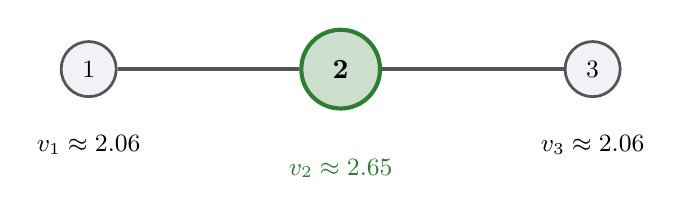
\begin{tikzpicture}[scale=1.0,
    leaf/.style={circle, draw=midgray, fill=boxfill, line width=1pt, minimum size=0.7cm, inner sep=0pt, font=\small},
    cent/.style={circle, draw=accentgreen, fill=accentgreen!25, line width=1.5pt, minimum size=1.0cm, inner sep=0pt, font=\bfseries}]
    \node[leaf] (n1) at (-3.2,0) {1};
    \node[cent] (n2) at (0,0) {2};
    \node[leaf] (n3) at (3.2,0) {3};
    \draw[midgray, line width=1.2pt] (n1)--(n2);
    \draw[midgray, line width=1.2pt] (n2)--(n3);
    \node[below=10pt, font=\small] at (n1.south) {$v_1 \approx 2.06$};
    \node[below=14pt, font=\small, accentgreen] at (n2.south) {$v_2 \approx 2.65$};
    \node[below=10pt, font=\small] at (n3.south) {$v_3 \approx 2.06$};
\end{tikzpicture}
\end{center}

\vspace{14pt}

\resultbox[boxfillgreen]{accentgreen}{%
    {\small Targeting node 2 costs $1/v_2 \approx 0.378$. Targeting a leaf costs $1/v_1 \approx 0.486$.}\\[3pt]
    {\color{accentgreen}\bfseries Centrality premium: $28.6\%$.}
}
\end{frame}

% ============================================================
% SLIDE 15: Bridge -- voting isn't linear
% ============================================================
\begin{frame}{Real voting isn't linear}
\accentline
\vspace{10pt}
\begin{columns}[T]
    \begin{column}{0.62\textwidth}
        \vspace{12pt}
        {\small Real institutions don't aggregate effort linearly.}

        \vspace{12pt}

        {\small Replace the linear rule $\sum_i a_i \geq \bar T$ with}
        \[
            \textstyle\sum_i f(a_i^*) \;\geq\; K
        \]
        {\small for some $C^2$ strictly increasing $f$.}
    \end{column}
    \begin{column}{0.36\textwidth}
        \begin{center}
        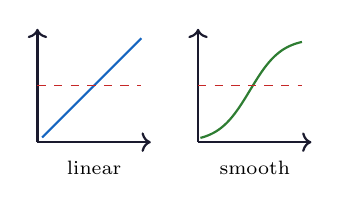
\begin{tikzpicture}[scale=0.6]
            % linear panel
            \draw[->, thick, darktext] (0,0) -- (2.4,0);
            \draw[->, thick, darktext] (0,0) -- (0,2.4);
            \draw[thick, accentblue] (0.1,0.1) -- (2.2,2.2);
            \draw[dashed, accentred] (0,1.2) -- (2.2,1.2);
            \node[below, font=\scriptsize] at (1.2,-0.2) {linear};
            % sigmoid panel
            \begin{scope}[xshift=3.4cm]
                \draw[->, thick, darktext] (0,0) -- (2.4,0);
                \draw[->, thick, darktext] (0,0) -- (0,2.4);
                \draw[thick, accentgreen, smooth, samples=40, domain=0.05:2.2]
                    plot (\x, {2.2/(1+exp(-3*(\x-1.1)))});
                \draw[dashed, accentred] (0,1.2) -- (2.2,1.2);
                \node[below, font=\scriptsize] at (1.2,-0.2) {smooth};
            \end{scope}
        \end{tikzpicture}
        \end{center}
    \end{column}
\end{columns}
\end{frame}

% ============================================================
% SLIDE 16: Theorem 2 -- Slope-weighted Bonacich
% ============================================================
\begin{frame}{Theorem 2 --- Slope-weighted Bonacich}
\accentline
\vspace{6pt}

\resultbox[boxfillgreen]{accentgreen}{%
    {\color{accentgreen}\bfseries Theorem 2 (Slope-weighted concentration).}\\[3pt]
    {\small Let $f$ be $C^2$ with $f' > 0$, and let $a^0 = Mb$ be the no-lobbying equilibrium. Define the \emph{slope-weighted centrality}}
    \[
        w_j \;=\; \sum_i f'(a^0_i)\, M_{ij}, \qquad a^0 \;=\; M b.
    \]
    {\small As the support gap $\Delta = K - F(a^0) \downarrow 0$, the cost-minimizing plan concentrates on $j^* \in \arg\max_j w_j$.}
}

\vspace{8pt}

{\small\color{midgray}\bfseries Linear $f$ or $b = 0$:}\, {\small $w$ collapses to $v$. Theorem 1 recovered.}\\[4pt]
{\small\color{accentred}\bfseries Concave $f$ \,+\, nonzero $b$:}\, {\small ranking can flip --- fence-sitters can beat saturated central partisans.}
\end{frame}

% ============================================================
% SLIDE 17: Saturation flip (visual)
% ============================================================
\begin{frame}{The saturation flip}
\accentline
\vspace{4pt}
\begin{columns}[T]
    \begin{column}{0.48\textwidth}
        \begin{center}
        {\small\color{accentgreen}\bfseries $b = 0$: center wins}\\[4pt]
        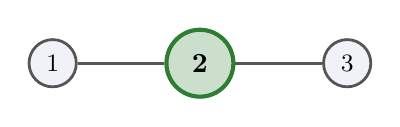
\begin{tikzpicture}[scale=0.85,
            leaf/.style={circle, draw=midgray, fill=boxfill, line width=1pt, minimum size=0.6cm, inner sep=0pt, font=\small},
            cent/.style={circle, draw=accentgreen, fill=accentgreen!25, line width=1.5pt, minimum size=0.85cm, inner sep=0pt, font=\bfseries}]
            \node[leaf] (n1) at (-2.2,0) {1};
            \node[cent] (n2) at (0,0) {2};
            \node[leaf] (n3) at (2.2,0) {3};
            \draw[midgray, line width=1pt] (n1)--(n2);
            \draw[midgray, line width=1pt] (n2)--(n3);
        \end{tikzpicture}
        \end{center}
        \vspace{4pt}
        {\footnotesize $w \approx (0.515,\, 0.662,\, 0.515)$}
    \end{column}
    \begin{column}{0.48\textwidth}
        \begin{center}
        {\small\color{accentred}\bfseries $b = 2$: leaves win}\\[4pt]
        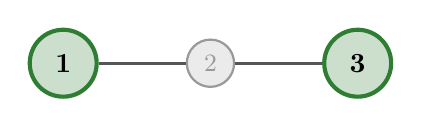
\begin{tikzpicture}[scale=0.85,
            leafw/.style={circle, draw=accentgreen, fill=accentgreen!25, line width=1.5pt, minimum size=0.85cm, inner sep=0pt, font=\bfseries},
            faded/.style={circle, draw=lightgray, fill=lightgray!20, line width=0.8pt, minimum size=0.6cm, inner sep=0pt, font=\small\color{lightgray}}]
            \node[leafw] (n1) at (-2.2,0) {1};
            \node[faded] (n2) at (0,0) {2};
            \node[leafw] (n3) at (2.2,0) {3};
            \draw[midgray, line width=1pt] (n1)--(n2);
            \draw[midgray, line width=1pt] (n2)--(n3);
        \end{tikzpicture}
        \end{center}
        \vspace{4pt}
        {\footnotesize $a^0 \approx (4.12,\, 5.29,\, 4.12)$ (saturated)}\\[2pt]
        {\footnotesize $w \approx (0.0261,\, 0.0259,\, 0.0261)$}
    \end{column}
\end{columns}

\vspace{10pt}

{\small\color{midgray} When the central member is saturated, peripheral fence-sitters become the cheaper target.}
\end{frame}

% ============================================================
% SLIDE 18: Model B -- Probabilistic votes
% ============================================================
\begin{frame}{Model B: probabilistic votes}
\accentline
\vspace{6pt}

{\small Now $a_i \in (0,1)$ is the probability member $i$ votes yes. Replace the quadratic cost with binary entropy. Best response is sigmoidal:}

\[
    a_i^* \;=\; \sigma\!\left(\frac{b_i + t_i + \beta \sum_j g_{ij}\, a_j^*}{\kappa}\right).
\]

\vspace{4pt}

\begin{center}
\[
    \tilde v_j \;=\; \underbrace{a_j^*(1 - a_j^*)}_{\text{swing slope}} \;\cdot\; \underbrace{\bigl[\text{modified Bonacich}\bigr]_j}_{\text{network propagation}}
\]
\end{center}

\vspace{6pt}

{\small The swing-voter slope $\sigma'(a^*)$ plays exactly the role of $f'(a^0)$ from Theorem 2 --- the slope-weighting channel is real.}
\end{frame}

% ============================================================
% SLIDE 19: Open directions + Thank you
% ============================================================
\begin{frame}{Open directions}
\accentline
\vspace{14pt}

{\small\color{accent}\bfseries 1.}\, {\small Directed networks: in-Bonacich (susceptibility) vs out-Bonacich (influence).}

\vspace{12pt}

{\small\color{accent}\bfseries 2.}\, {\small Competing lobbyists.}

\vspace{12pt}

{\small\color{accent}\bfseries 3.}\, {\small Repeated/dynamic game extension}

\vspace{30pt}

\begin{center}
{\small\color{midgray} Thank you. Questions?}
\end{center}
\end{frame}

\end{document}
